\documentclass{article}
\usepackage{listings}
\usepackage[margin=1in]{geometry}
\usepackage{graphicx}

\title{CMOR 421/521, Homework \#1: \LaTeX{} Submission}
\author{\texttt{amc50}}
\date{March 7, 2024}

\begin{document}
\maketitle

\section{Compilation}

\subsection{Accessing NOTS Cluster}
It is important to note that the following process is done on Rice Owls Network. This is the case as the cluster login requires accessing through a Secure Shell on the Rice campus network.

\bigskip
\noindent Command used to ssh into NOTS:

\begin{verbatim}
MacBook-Pro-95:cmor-421-521-submissions antoniocrivello$ ssh amc50@nots.rice.edu
\end{verbatim}

\bigskip
\noindent Command used to activate interactive node on NOTS:
\begin{verbatim}
[amc50@nlogin1 ~]$ srun --pty --partition=interactive --ntasks=1 --mem=1G --time=00:30:00 $SHELL
\end{verbatim}

\bigskip
\noindent Command used to load modules needed for compilation:
\begin{verbatim}
[amc50@bc9u7n1 ~]$ module load GCC/13.1.0 
\end{verbatim}

\bigskip
\noindent To access files created on local desktop, a GitHub repository is used. As such, this repository must be cloned on the cluster. This process requires a password-protected key.

\bigskip
\noindent Command used to generate SSH key :
\begin{verbatim}
[amc50@bc9u7n1 ~]$ ssh-keygen -t ed25519 -C "amc50@rice.edu"
\end{verbatim}

\bigskip
\noindent Command used to access public key:
\begin{verbatim}
[amc50@bc9u7n1 ~]$ emacs ~/.ssh/id_ed25519.pub 
\end{verbatim}

\bigskip
\noindent After accessing the SSH key, it is added to list of SSH keys on GitHub.

\bigskip
\noindent Command used to clone cmor-421-521-submissions GitHub repository:
\begin{verbatim}
[amc50@bc9u7n1 ~]$ git clone git@github.com:AntonioCrivello/cmor-421-521-submissions.git    
\end{verbatim}

\bigskip
\noindent For compilation on the NOTS Cluster I am utilizing a Makefile. 

\bigskip
\noindent Set of commands to compile project: 
\begin{verbatim}
[amc50@bc9u7n1 homework-1]$ make clean
rm -rf matmul_recursive 

[amc50@bc9u7n1 homework-1]$ make
g++ main.cpp -O3 -std=c++11 -o matmul_recursive
\end{verbatim}

\bigskip
\noindent In order to efficiently generate timings for matrix sizes of n = $2^{i}$ for i = 4,5,6 ... 10, I have created a Bash script to run the aforementioned make clean and make commands with the matrix size as an argument. Additionally, to determine the optimal block size for the block size dependent matrix-matrix multiplication methods these are also supplied as an argument to the executable. After initial testing it was observed that block sizes that are too large exhibited no improvement in the methods. For this reason block sizes above 256 are excluded from the rest of the report.

\bigskip
\noindent Command used to generate timings and compile project:
\begin{verbatim}
[amc50@bc9u7n1 homework-1]$ ./generate-timings.sh 
\end{verbatim}

\section{Matrix-Matrix Multiplication}

\subsection{Column Major Storage for Matrix-Matrix Multiplication}
If the matrices involved in matrix-matrix multiplication were stored in column major format instead of row major format, consecutive elements within a row are no longer stored contiguously. As such, the structuring of the matrix-matrix multiplication is unable to take advantage of the cache locality and efficient memory accessing of elements in a row as the current implementation has it. To adjust for this, instead, the implementation needs to change so that the elements within a column are contiguously accessed to still benefit from memory locality. The simplest way to accomplish this is to change the loop order used during the matrix-matrix multiplication. Using the naive implementation as an example, the current implementation has the outer loop populate the rows of matrix \( C \) contiguously. To achieve this, the middle loop iterates over the columns of the matrix \( C \) on that row and the inner loop iterates over the elements within the row of matrix \( A \) and the column of matrix \( B \). For the column-major version, the loop order should change so that the outer loop iterates through the columns of matrix \( C \), middle loop through the rows, and the inner loop iterates within each column of matrix \( A \) and within each row of matrix \( B \). This will allow the required data values to be located adjacent to each other. Additionally, there is a potential benefit in unrolling the innermost loop to reduce overhead and utilize the location of the column values more effectively. 

\subsection{Matrix Transpose}
When matrices are stored in column-major format, it is excepted that performing the operation $A^{T}B$ would be faster than \( AB\). The primary reason this is the case is because when applying the transpose to matrix \( A\) and then multiplying to matrix \( B\), the matrix-matrix multiplication involves iterating through the rows of $A^{T}$ and the columns of \( B\). Given then that A is stored in column-major format, transposing it results in the columns becoming the rows, ensuring contiguous memory access. Consequently, both $A^{T}$ and \( B \) benefit from contiguous memory access, which is an improvement over the singular contiguous memory access possible for \(AB \) in row-major format. Conversely, if the matrices are stored in row-major format, $A^{T}B$ is expected to be slower than \(AB \). This is because neither matrix would benefit from contiguous memory access, leading to iterations through the columns of \( A\) and columns of \( B\).
\clearpage

\section{Optimizing Matrix-Matrix Multiplication}

\subsection{Naive Matrix-Matrix Multiplication Timing}

\begin{table}[ht!]
    \caption{Naive Matrix-Matrix Multiplication Timings (Seconds) on NOTS}
    \centering
    \resizebox{\textwidth}{!}{%
    \begin{tabular}{|c|c|c|c|c|c|c|c|}
        \hline
        \multicolumn{1}{|c|}{} & \multicolumn{7}{c|}{Block Size} \\
        \cline{2-8}
        \multicolumn{1}{|c|}{Matrix Size} & 4 & 8 & 16 & 32 & 64 & 128 & 256 \\
        \hline
        n = 16 & 3.07974e-06 & 3.079e-06 & 3.0788e-06 & & & & \\
        \hline
        n = 32 & 2.50003e-05 & 2.35716e-05 & 2.53559e-05 & 2.51123e-05 & & & \\
        \hline
        n = 64 & 0.000207474 & 0.000206754 & 0.000208333 & 0.000199271 & 0.000199479 & & \\
        \hline
        n = 128 & 0.0019859 & 0.00196828 & 0.00191194 & 0.00192037 & 0.00194726 & 0.00197747 & \\
        \hline
        n = 256 & 0.0279104 & 0.0280141 & 0.0287367 & 0.0287943 & 0.028138 & 0.0279499 & 0.0287771 \\
        \hline
        n = 512 & 0.233498 & 0.233413 & 0.233334 & 0.233284 & 0.233584 & 0.233391 & 0.233356 \\
        \hline 
        n = 1024 & 1.84701 & 1.8472 & 1.84773 & 1.84869 & 1.85021 & 1.84724 & 1.84663 \\
        \hline
    \end{tabular}
    }
\end{table}


\subsection{Blocked Matrix-Matrix Multiplication Timing}
\begin{table}[ht!]
    \caption{Blocked Matrix-Matrix Multiplication Timings (Seconds) on NOTS}
    \centering
    \resizebox{\textwidth}{!}{%
    \begin{tabular}{|c|c|c|c|c|c|c|c|}
        \hline
        \multicolumn{1}{|c|}{} & \multicolumn{7}{c|}{Block Size} \\
        \cline{2-8}
        \multicolumn{1}{|c|}{Matrix Size} & 4 & 8 & 16 & 32 & 64 & 128 & 256 \\
        \hline
        n = 16 & 5.19284e-06 & 3.51702e-06 & 3.50028e-06 & & & & \\
        \hline
        n = 32 & 3.67851e-05 & 2.57295e-05 & 2.7263e-05 & 2.5416e-05 & & & \\
        \hline
        n = 64 & 0.00028435 & 0.000220714 & 0.000204823 & 0.000191006 & 0.000204107 & & \\
        \hline
        n = 128 & 0.002123 & 0.00163014 & 0.00151718 & 0.00148115 & 0.00209127 & 0.00193627 & \\
        \hline
        n = 256 & 0.0192998 & 0.0136306 & 0.0122848 & 0.0155541 & 0.0169318 & 0.0214555 & 0.0289351 \\
        \hline
        n = 512 & 0.158257 & 0.111171 & 0.118842 & 0.156956 & 0.199324 & 0.23294 & 0.233945 \\
        \hline
        n = 1024 & 1.22181 & 0.881711 & 0.934548 & 1.2512 & 1.93896 & 1.8779 & 1.85881 \\
        \hline
    \end{tabular}
    }
\end{table}


\subsection{Discussion}

As exhibited by the results in Table 2, the block size is independent of the size of the matrix. This consistently aligns with the principle behind the Blocked Matrix-Matrix method, which aims to take advantage of the machine's cache. By dividing the matrix of size n into N sub-matrices that fit within the fast memory, cache utilization is maximized. As such, the optimal block size depends on the size of the fast memory rather than the size of the matrix itself. Based on timing analysis, the optimal block size is determined to be \( b\) = 8. It is important to note that there are some minor fluctuations in the optimal block size between \( b\) = 8 and \( b\) = 16; however, this is likely due to inconsistencies in the timings. The optimal block size stabilizes for larger computations as the overall timings are greater, meaning that minor timing differences have less influence on the overall average.

\subsection{Roofline Plot Results}

For the following roofline plots, the computations were run on the NOTS Cluster Intel(R) Xeon(R) CPU E5-2650 v2 @ 2.60Hz. For this specific processor the CPU specifications are a max performance of 166.4 GFLOPS and max memory bandwidth of 59.7 GB/s. Considering only one core for this model and with the processor having 8 cores, the peak performance per core is 20.8 GFLOPS. To determine the theoretical limit, the roofline is defined as the minimum between the peak performance and the computational intensity (CI) multiplied by the peak bandwidth. Each experimental data point on the plot represents the the operational intensity in FLOPS/byte versus the performance in GFLOPS/s. For the naive implementation, the operational intensity is determined by calculating CI using equation (1). Additionally, the GFLOPS/s is based on the experimentally measured run times. The blocked method is evaluated in the same manor, but in this case, it utilizes the CI defined by (2). In this equation, \(b \) is the block size used for tiling the matrix.

\begin{equation}
CI = \frac{2 \cdot n^{3}}{(3 \cdot n^{2} + n^{3}) * 8}
\end{equation}

\begin{equation}
CI = \frac{2 \cdot n^{3}}{(2 \cdot n^{2} + \frac{2 \cdot n^{3}}{b}) * 8}
\end{equation}

%\clearpage

\begin{figure}[!htb]
    \centering
    \fbox{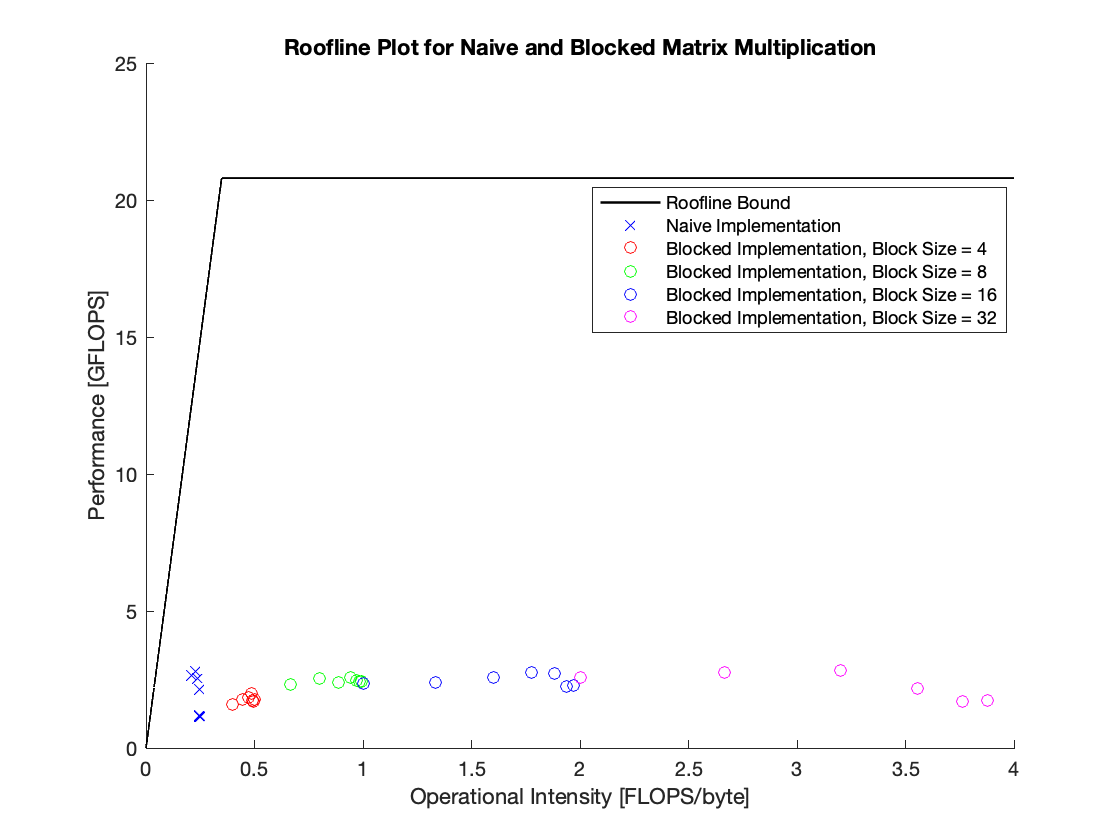
\includegraphics[width=0.8\linewidth]{naive_and_blocked_roofline.png}}
    \caption{Roofline Plot for Naive and Blocked Matrix-Matrix Multiplication}
\end{figure}

\section{Recursive Matrix-Matrix Multiplication}

In my implementation of Recursive Matrix-Matrix multiplication, I have two versions. In the first version, if the matrix is smaller than the block size, no intermediate doubles are allocated when running the "microkernel." Instead, the writing to memory for \(C \) is done directly at the inner loop every time. In the second versions, doubles are allocated and then writing to \(C \) occurs at the completion of the inner loop. While it is not substantial, it remains interesting to observe the difference in performance. 

\subsection{Timing}
\begin{table}[ht!]
    \caption{Recursive Matrix-Matrix Multiplication Timings (Seconds) on NOTS}
    \centering
    \resizebox{\textwidth}{!}{%
    \begin{tabular}{|c|c|c|c|c|c|c|c|}
        \hline
        \multicolumn{1}{|c|}{} & \multicolumn{7}{c|}{Block Size} \\
        \cline{2-8}
        \multicolumn{1}{|c|}{Matrix Size} & 4 & 8 & 16 & 32 & 64 & 128 & 256 \\
        \hline
        n = 16 & 4.85776e-06 & 4.30824e-06 & 4.22884e-06 & & & & \\
        \hline
        n = 32 & 3.52447e-05 & 3.0559e-05 & 3.19342e-05 & 3.66818e-05 & & & \\
        \hline
        n = 64 & 0.000287541 & 0.00025944 & 0.000257827 & 0.000282055 & 0.000266902 & & \\
        \hline
        n = 128 & 0.0022258 & 0.00219709 & 0.0023011 & 0.00261993 & 0.00293102 & 0.00291156 & \\
        \hline
        n = 256 & 0.0189461 & 0.0195265 & 0.0213893 & 0.026722 & 0.0291919 & 0.0315255 & 0.0346263 \\
        \hline
        n = 512 & 0.172671 & 0.180503 & 0.249633 & 0.299008 & 0.328264 & 0.337827 & 0.353049 \\
        \hline
        n = 1024 & 1.32852 & 1.41536 & 1.9797 & 2.38446 & 2.58796 & 2.60521 & 2.61198 \\
        \hline
    \end{tabular}
    }
\end{table}

\begin{table}[ht!]
    \caption{Recursive with Intermediates Matrix-Matrix Multiplication Timings (Seconds) on NOTS}
    \centering
    \resizebox{\textwidth}{!}{%
    \begin{tabular}{|c|c|c|c|c|c|c|c|}
        \hline
        \multicolumn{1}{|c|}{} & \multicolumn{7}{c|}{Block Size} \\
        \cline{2-8}
        \multicolumn{1}{|c|}{Matrix Size} & 4 & 8 & 16 & 32 & 64 & 128 & 256 \\
        \hline
        n = 16 & 4.45684e-06 & 4.08408e-06 & 3.1788e-06 & & & & \\
        \hline
        n = 32 & 3.50298e-05 & 3.05299e-05 & 3.15184e-05 & 2.54159e-05 & & & \\
        \hline
        n = 64 & 0.000278312 & 0.000262585 & 0.00025788 & 0.000290819 & 0.000209489 & & \\
        \hline
        n = 128 & 0.00221864 & 0.00219514 & 0.00229489 & 0.0026175 & 0.00293402 & 0.00192901 & \\
        \hline
        n = 256 & 0.0189665 & 0.0195024 & 0.0213916 & 0.0266558 & 0.0292192 & 0.0310885 & 0.0287829 \\
        \hline
        n = 512 & 0.172988 & 0.180603 & 0.249605 & 0.298945 & 0.328335 & 0.326461 & 0.353065 \\
        \hline
        n = 1024 & 1.32819 & 1.41644 & 1.98067 & 2.38451 & 2.58734 & 2.60538 & 2.61249 \\
        \hline
    \end{tabular}
    }
\end{table}

\subsection{Optimizing Recursive Matrix-Matrix Multiplication}
For the Recursive Matrix-Matrix Multiplication method, the optimal block size is 8, matching the Blocked Matrix-Matrix multiplication method. Given that these methods are executed on the same CPU with the identical fast cache configurations this makes sense. It is important to note that again the optimal block size does slightly vary between 8 and 16, but is again attributed to potential inconsistent timings. 

\subsection{Implementation Check}
In order to confirm the correctness of the Recursive Matrix-Matrix Multiplication method, matrices \( A \) and \( B \) are initialized to the identity matrix. The matrices are then multiplied together, and the resulting matrix \( C \) is expected to be equal to the identity matrix \( I \). To verify that \( C \) is indeed equal to \( I \) up to machine precision, an element-wise comparison is performed, and the absolute difference between corresponding elements of \( C \) and \( I \) is computed. These differences are accumulated, and if the sum exceeds \( 1 \times 10^{-15} \times n \), where \( n \) is the size of the matrix, it indicates that the matrices are not identical. It is important to note that the scaling is included due to numerical round-off. If the sum is within this allowable tolerance, the method has been correctly implemented. In my implementation, this equality check is performed after each call of a matrix-matrix multiplication function.

\subsection{Roofline Plot Results}

As described previously, the roofline plot requires calculating the computational intensity (CI). For the recursive implementation this is defined be equation (3). Otherwise, the process is identical as before. 

\begin{equation}
CI = \frac{2}{3 * 8} \cdot b 
\end{equation}

\clearpage

\begin{figure}[!htb]
    \centering
    \fbox{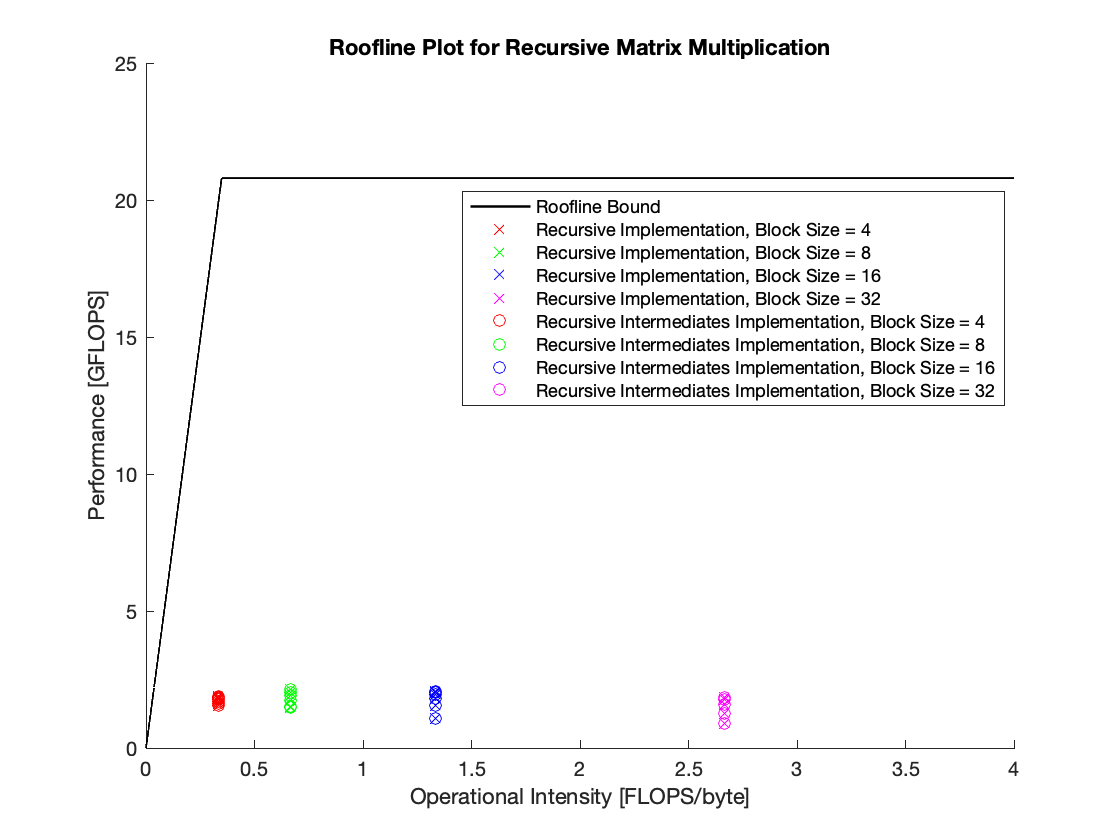
\includegraphics[width=0.8\linewidth]{recursive_roofline.png}}
    \caption{Roofline Plot for Recursive Matrix-Matrix Multiplication}
\end{figure}

\subsection{Discussion}
The performance of the Recursive Matrix-Matrix multiplication method was consistently outperformed by that of the optimized Blocked Matrix-Matrix multiplication. Several factors likely contribute to this observed difference. One significant reason is the increased overhead resulting from the eight function calls per dividing the block size in half necessary for the recursive method. This is compared to the blocked method which does not require additional function calls but requires additional iterations instead. Additionally, the blocked method demonstrated the closest performance to the roofline bound among the three implementations, with the recursive method following and the naive method performing the worst. This difference can largely be attributed to the enhanced efficiency and thus reduced runtime of the blocked method. As expected, there was not much difference between the two recursive approaches. While the intermediate version showed a slight improvement with larger matrices it was relatively negligible. Lastly, despite the recursive method being slower than the blocked method, it still offers an important advantage. The trade-off for its slower speed is being cache-oblivious, compared to the blocked method which requires knowledge about the cache to implement. This freedom can be valuable in more complex situations.

\end{document}

